%!TEX TS-program = xelatex

\documentclass[aspectratio=169]{beamer}

\newbool{russian}
\booltrue{russian}
\usepackage{HSE-theme/beamerthemeHSE}

\usepackage[english,russian]{babel}
\usepackage{amsmath}
\usepackage[no-math]{fontspec}
\IfFontExistsTF{HSE Sans}{
    \setsansfont{HSE Sans}
}{
    \setsansfont{CMU Sans Serif}
}
\IfFontExistsTF{Courier New}{
    \setmonofont{Courier New}
}{
    \setmonofont{Latin Modern Mono}
}

\uselanguage{russian}
\languagepath{russian}
\deftranslation[to=russian]{Theorem}{Теорема}
\deftranslation[to=russian]{Definition}{Определение}
\deftranslation[to=russian]{Definitions}{Определения}
\deftranslation[to=russian]{Corollary}{Следствие}
\deftranslation[to=russian]{Fact}{Факт}
\deftranslation[to=russian]{Example}{Пример}
\deftranslation[to=russian]{Examples}{Примеры}

\usepackage{graphicx}
\usepackage{booktabs}
\usepackage{array}

\graphicspath{{figures/}{graphics/}}

\title[Предлагаемый подход]{Предлагаемый подход к последующему GRPO-дообучению text-to-MIDI}
\subtitle{Материал по разделу ``Предлагаемый подход''}
\author[Курсовой проект]{Автор курсовой работы}
\institute{Факультет компьютерных наук НИУ ВШЭ}
\date{2026}

\begin{document}

\frame[plain]{\titlepage}

\begin{frame}
\frametitle{Почему нужно последующее дообучение}
\begin{itemize}
    \item Базовая text-to-MIDI модель учится предсказывать следующий токен, но это не гарантирует качество всего музыкального фрагмента.
    \item Для итогового MIDI важны глобальные свойства: тональная согласованность, ритмическая устойчивость, фактура и соответствие текстовому описанию.
    \item Один запрос допускает несколько корректных музыкальных реализаций, поэтому обучение по одному эталону ограничено.
    \item Нужна схема, которая сравнивает несколько сгенерированных кандидатов и усиливает более удачные.
\end{itemize}
\end{frame}

\begin{frame}
\frametitle{Общая идея подхода}
\begin{enumerate}
    \item Берём уже обученный генератор text-to-MIDI.
    \item Для одного текстового запроса генерируем группу MIDI-кандидатов.
    \item После декодирования оцениваем каждый кандидат правилами, критиком или их комбинацией.
    \item Считаем относительное преимущество кандидатов внутри группы.
    \item Обновляем модель в сторону более предпочтительных ответов с помощью GRPO.
\end{enumerate}

\medskip
\begin{alertblock}{Ключевая особенность}
Награда вычисляется не на уровне отдельного токена, а по завершённой MIDI-последовательности.
\end{alertblock}
\end{frame}

\begin{frame}
\frametitle{Базовая модель Text2midi}
\begin{columns}
\column{0.53\textwidth}
\begin{itemize}
    \item Исходный генератор рассматривается как условная политика $\pi_\theta(y \mid x)$.
    \item Вход: текстовый запрос с описанием жанра, настроения, темпа, размера и инструментов.
    \item Выход: авторегрессионно сгенерированная последовательность музыкальных токенов, которая затем декодируется в MIDI.
    \item Базовая модель уже умеет порождать валидные MIDI, но может создавать лишние дорожки, переуплотнённую фактуру и слабое соответствие запросу.
\end{itemize}

\column{0.47\textwidth}
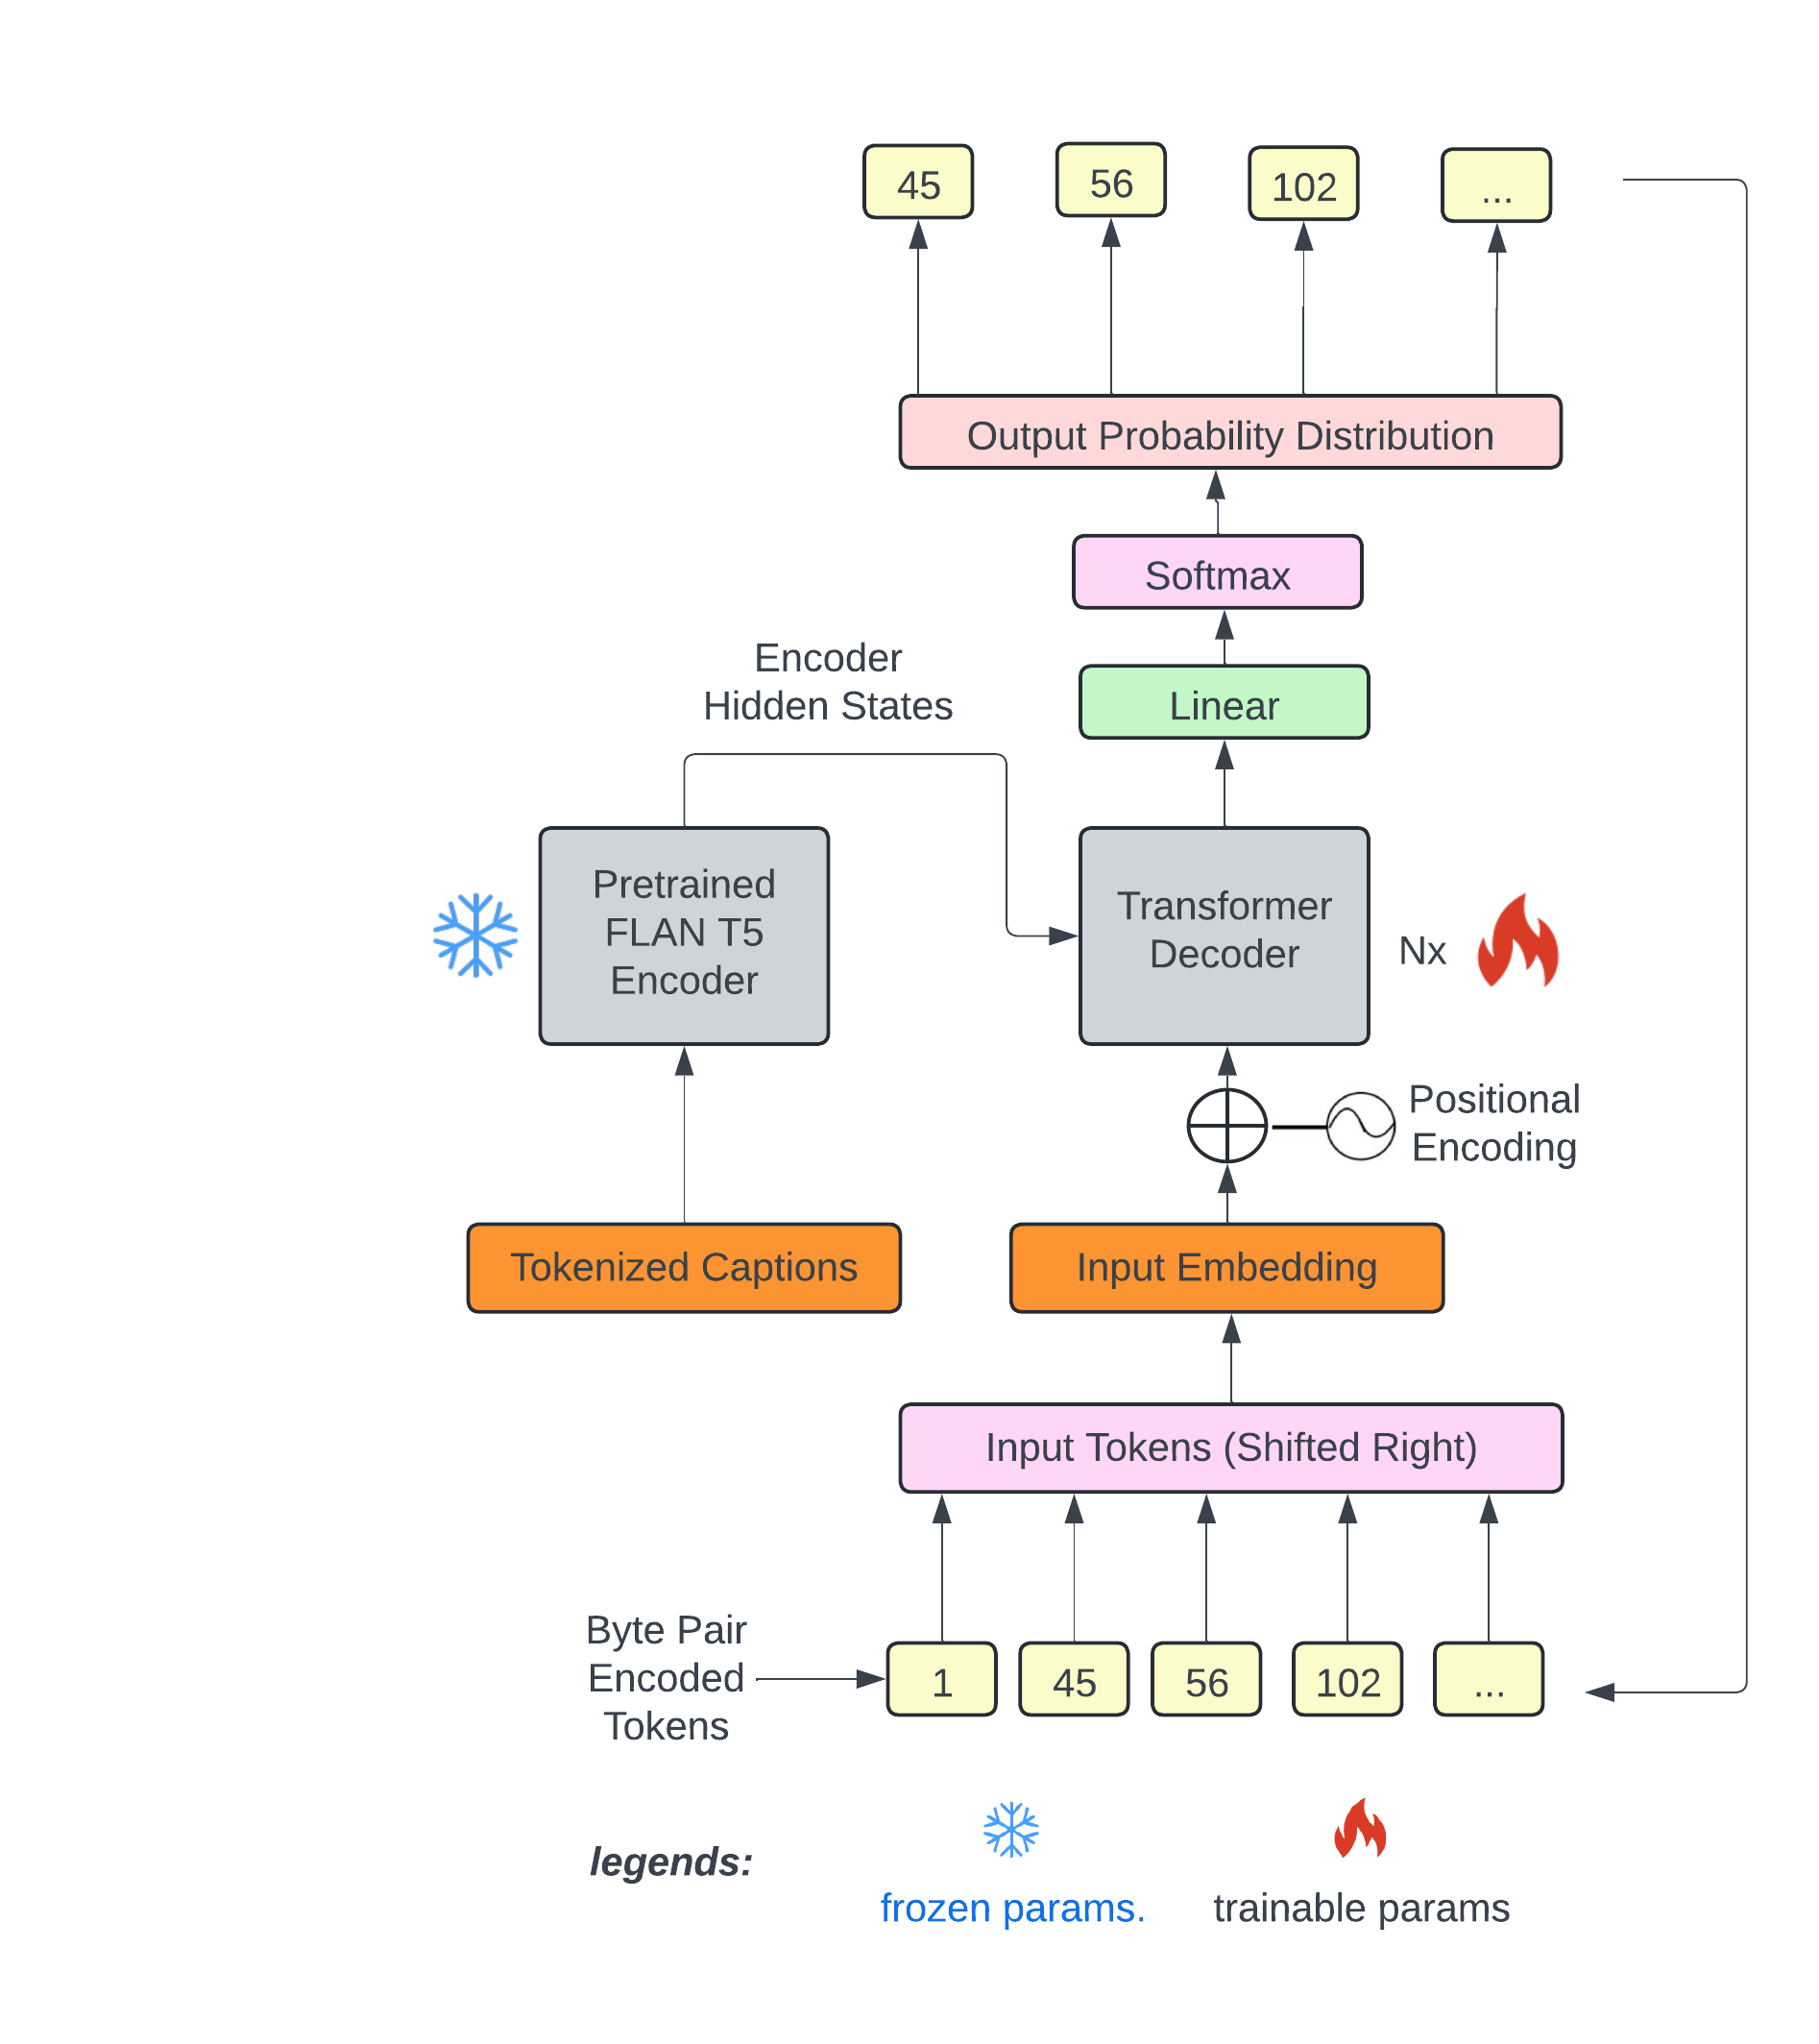
\includegraphics[width=\linewidth]{text2midi/text2midi_architecture.jpg}
\end{columns}
\end{frame}

\begin{frame}
\frametitle{GRPO как схема дообучения}
\small
Для запроса $q$ генерируется группа ответов
\[
\{o_i\}_{i=1}^G \sim \pi_{\theta_{\mathrm{old}}}(O \mid q),
\qquad
r_i = R(q, o_i).
\]

Относительное преимущество вычисляется внутри группы:
\[
\hat{A}_i = \frac{r_i - \bar{r}}{s_r + \varepsilon_A},
\qquad
\bar{r} = \frac{1}{G}\sum_{j=1}^G r_j.
\]

Оптимизируется clipped-цель с KL-регуляризацией к опорной модели:
\[
\mathcal{L}_{\mathrm{GRPO}} \propto
\sum_{i,t} m_{i,t}
\left(
-\min(\rho_{i,t}(\theta)\hat{A}_i,\,
\operatorname{clip}(\rho_{i,t}(\theta),1-\epsilon,1+\epsilon)\hat{A}_i)
+ \beta D_{i,t}
\right).
\]

\begin{itemize}
    \item Если кандидат лучше среднего по группе, вероятность его токенов увеличивается.
    \item KL-регуляризация не даёт модели слишком далеко уйти от исходного генератора.
\end{itemize}
\end{frame}

\begin{frame}
\frametitle{Один шаг обучения}
\small
\begin{tabular}{p{0.08\textwidth} p{0.30\textwidth} p{0.50\textwidth}}
\toprule
\textbf{Этап} & \textbf{Операция} & \textbf{Назначение} \\
\midrule
1 & Выбор запроса & Задаётся текстовое условие для группы кандидатов. \\
2 & Генерация кандидатов & Модель порождает несколько MIDI-вариантов для одного запроса. \\
3 & Декодирование & Токены преобразуются в музыкальное представление и MIDI-файл. \\
4 & Вычисление награды & Кандидаты оцениваются правилами, критиком или смешанной схемой. \\
5 & Нормировка в группе & Награды переводятся в относительные преимущества. \\
6 & Обновление GRPO & Обновляются обучаемые параметры с clip-ограничением и KL-регуляризацией. \\
\bottomrule
\end{tabular}

\medskip
Дополнительно сохраняются артефакты шага: тексты запросов, MIDI-файлы, компоненты награды, статистика валидности и чекпойнты модели.
\end{frame}

\begin{frame}
\frametitle{Что именно обучается}
\begin{columns}
\column{0.52\textwidth}
\begin{block}{Основной режим}
\textbf{LoRA-адаптация} в FFN-блоках декодера:
\begin{itemize}
    \item слои \texttt{linear1} и \texttt{linear2};
    \item меняется распределение музыкальных токенов;
    \item большая часть исходной модели остаётся замороженной.
\end{itemize}
\end{block}

\column{0.48\textwidth}
\begin{block}{Альтернатива}
\textbf{Прямое частичное дообучение} выбранных параметров:
\begin{itemize}
    \item сильнее меняет поведение модели;
    \item требует более осторожного выбора learning rate;
    \item сильнее зависит от контроля KL.
\end{itemize}
\end{block}
\end{columns}

\begin{exampleblock}{Ожидаемый эффект}
Сместить распределение генераций в сторону более музыкально согласованных и лучше соответствующих текстовому запросу MIDI-кандидатов.
\end{exampleblock}
\end{frame}

\begin{frame}
\frametitle{Итог}
\begin{itemize}
    \item Предлагаемый подход не переобучает модель с нуля, а надстраивает поверх готового text-to-MIDI генератора этап согласования.
    \item Качество задаётся внешней наградой по завершённому MIDI-фрагменту, а не только вероятностями токенов.
    \item GRPO позволяет использовать относительное сравнение нескольких кандидатов без отдельной модели ценности.
    \item Практический акцент сделан на устойчивом дообучении с ограниченным числом обучаемых параметров.
\end{itemize}
\end{frame}

\end{document}
